% !TEX root = ../../main.tex
\documentclass[../../main.tex]{subfiles}

\begin{document}

\subsection{Processing}
Data systems can be classified into three types by data access patterns and processing
\begin{itemize}
    \item Online systems.
    \item Batch processing systems.
    \item Streaming processing systems.
\end{itemize}
Online systems fetchs/process small amounts of data constantly usually on transactional
systems. Batch processing systems fetch vast amounts of data on a schedule, process it
and store it for later use. Streaming processing systems is an intermediate state
between batch processing and online systems.

UNIX tools is an example of well design that have been used for decades and still
relevant for many use cases. UNIX phylosophy encourage programmer
\begin{itemize}
    \item Files is the common input/output interface whether it is a unix socket
        a device, a file, stdin or stdout.
    \item Create specialize well written and optimal programs to do a single task.
    \item Do not extend tools, rather create another.
    \item The input of an specific job is the output of another.
\end{itemize}
This set of rules can be summarized and extended to other frameworks as
\begin{itemize}
    \item Separate logic from wiring.
    \item Source data and intermediate states should be immutable.
\end{itemize}


\subsection{Reliability, Scalability and Mantainability}
\begin{definition}[Reliability]
    Keep working with hardware, software and human errors. To implement is important to decouple and isolate components, seek faults over failure, make easy to do the right thing and discourage the wrong, make fast to roll back changes.
\end{definition}
\begin{definition}[Scalability]
    Reasonable ways to deal with grows. To implement reliability is important to describe with metrics.
\end{definition}
\begin{definition}[Maintainability]
    It is divided into three parts
    \begin{itemize}
        \item Operability: Make operations easy. To implement track problem causes, automate deployment, define process.
        \item Simplicity: Easy for new engineers to understand. To implement seek abstraction over hardcode.
        \item Evolvability: Make easy for engineers to make changes.
    \end{itemize}
\end{definition}


\subsection{Database internals}
\begin{itemize}
    \item Elements
    \begin{itemize}
        \item Row id: Database internal id for each row, possibly independent of business id
        \item Page: Fundamental unit of storage. Can store tables, rows, columns, indexes, sequences, documents, etc. Pages are read by filename, by offset and by length and this is why fixed size data types is better than variable lenght size data types.
        \item Primary key: Piece of data that uniquely identifies it.
        \item Heap: Structure to store tables as pages
        \item Index: Structure that enhance data access
    \end{itemize}
\end{itemize}
Types of databases
\begin{center}
    \begin{tabular}{ |c|c|c| }
    \hline
    & Row store & Column store \\
    \hline
    \hline
    System type & OLTP & OLAP \\
    \hline
    Optimize for & Read/Write & Aggregation/Compression \\
    \hline
    Slow at & Aggregation/Compression & Read/Write \\
    \hline
    Multicolumns & Efficient & Inefficient \\
    \hline
    \end{tabular}
\end{center}


\subsection{Databases - ACID}
\begin{definition}[Transaction]
    Collection of queries treated as a unit of work.
    \begin{itemize}
        \item Usually for insert and modify data.
        \item For read only transaction you can keep consistency.
        \item Use keywords BEGIN, COMMIT and ROLLBACK.
    \end{itemize}
\end{definition}

\begin{definition}[Atomicity]
    All queries in a transaction must succeed, otherwise all prior successfull queries must be rollback.
\end{definition}

\begin{definition}[Consistency]
    Refers to different parts of the data retrieving different information.
    \begin{itemize}
        \item Consistency in data: Referential integrity and business logic
        \item Consistency in reads: Retrieve the latest change as soon as committed.
        \begin{itemize}
            \item Eventual consistency
            \item Strong consistency
        \end{itemize}
    \end{itemize}
\end{definition}


\begin{definition}[Isolation]
    When multiple transactions read and write at the same time, inconsistency in the
    share data may arise. Therefore, run transactions in isolation one from others is
    very important
\end{definition}
Isolation is easy to handle for single thread applications, however accesing it in
concurrent mode may arise so called raced conditions:
\begin{itemize}
    \item Dirty reads:
        A transaction reads data modified by other transactions, but not yet committed
    \item Dirty writes:
        A transaction write data modified by other transactions, but not yet committed
    \item Read skew aka non repeatable reads:
        A transaction reads data from multiple rows before and after being modified and
        committed by other transactions(same row ids are retrieve with different values)
    \item Lost updates:
        One transaction's update to a record is overwritten by another transaction's
        update. Usually appears on read modify write patterns
    \item Write skew:
        A transaction updates a row based upon stale data
    \item Phantom reads:
        A transaction reads a set of rows and then new rows appear that were not present
        during the first read
\end{itemize}
To adress this problem we can implement either weak isolation levels(solve only a subset
of the isolation problems) or serializable isolation aka strong isolation levels (solve
all isolation problems):
\begin{itemize}
    \item Weak isolation levels:
    \begin{itemize}
        \item Read uncommitted
        \item Read committed
        \item Reapetable read
        \item Snapshot isolation
    \end{itemize}
    \item Strong isolation
\end{itemize}
each of these levels have multiple implementations. For serializable isolation exists
three main options
\begin{itemize}
    \item Actual serial execution
    \item Two phase locking(2PL) or pessimistic locking
    \item Serializable snapshot isolation or optimistic locking
\end{itemize}
Actual serial execution is run in a single thread. Two phase locking is a serializable
isolation implementation that consists in two types of locks:
\begin{itemize}
    \item Exclusive locks: prevent other process to access
    \item Share locks: prevent exclusive locks and data modification
\end{itemize}
Serializable snapshot isolation only check for serializable execution when the
transaction wants to commit, allowing transactions to proceed without blocking.


\begin{definition}[Durability]
    Changes made by committed transactions must be persisted in a durable non-volatile storage
    \begin{itemize}
        \item Write ahead log
        \item Asynchoronous snapshot
        \item Append only file
    \end{itemize}
\end{definition}


\subsection{Database Indexing}
A table in a relational database is store in a heap composed of multiple pages.
An index is a structure created outside the heap to provide a different access mechanism.
The order in which data is stored in heap is called physical order, while the order in
which data is stored in a index is called logical order. The main data structure used to
create indexes is called B+Tree which is a self-balancing tree with its leaf nodes
connected as a double linked list. The index contains exclusivelly the columns that it
was defined; the leftmost column, as the first sorting criteria and the rightmost
column, as the last sorting criteria. To include other columns not to be used for order,
but for access it should be added as a non key column.
\begin{figure}
    \centering
    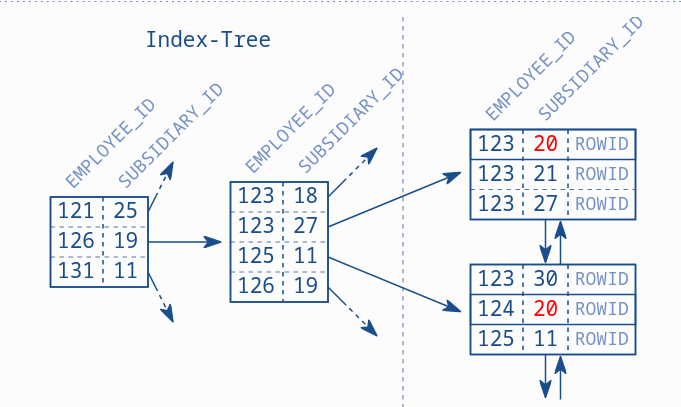
\includegraphics[width=0.7\textwidth]{btree}
    \caption{\href{https://use-the-index-luke.com/sql/where-clause/the-equals-operator/concatenated-keys}{B-Tree}}
\end{figure}
\begin{itemize}
    \item Types of indexes
    \begin{itemize}
        \item Primary index: Also known as clustered index, is a structure to store data in order usually by a primary key
        \item Secondary index: Also known as non clustered index, is an structure that provides an alternative way to access data
        \item Unique indexes
        \item Single column indexes
        \item Multi column index
        \item Bitmap index
        \item B-Tree index
        \item Function-based index
        \begin{itemize}
            \item Precomputed columns as workaround
            \item Only deterministic functions must be used
        \end{itemize}
    \end{itemize}
    \item Slow queries causes
    \begin{itemize}
        \item Not using indexes: full table scan
        \item Incorrect index design
        \begin{itemize}
            \item Long index range prefer to use full table scan
            \item Data skew: fetch many rows individually
            \item Fetch data: mainly from heap
        \end{itemize}
    \end{itemize}
    \item Tips
    \begin{itemize}
        \item Combining indexes avoid creating multiple distinct bitmap indexes
        \item Over indexing induce overhead on update/delete/insert
        \item Use non-key columns in indexes for common access patterns
        \item Index must use leftmost subset of columns
    \end{itemize}
    \item Index related operations
    \begin{itemize}
        \item Index only scan: hit index
        \item Index unique scan: retrieves single row, hit index and heap
        \item Index range scan: retrieves multiple rows, hit index and heap
        \item full table scan: hit heap
    \end{itemize}
\end{itemize}


\subsection{Database partitioning}
Partition is a technique storage systems that split data, possibly different machines,
to enhance scalability, reliability and improve performance for specific types of
queries by reducing the number of data that needs to be read. There are three main
strategies:
\begin{itemize}
    \item By hash
    \item By value
    \item By range
\end{itemize}
When the data is split across multiple servers it's called sharding


\subsection{Databases replication}
Replication is a technique in distributed systems that consists in data duplication
across nodes mainly, aiming for scalability, durability and availability. There are
three main strategies:
\begin{itemize}
    \item Leader - follower
    \item Multileader
    \item Leaderless
\end{itemize}
On a leader follower architecture writes are handle by a single central node, called
leader, which handles replication to the other nodes, called followers. On a multi
leader architecture, writes can be handle by multiple nodes. Finally, on leaderless
architecture all writes can be handle by all nodes without a specific leader.

Data changes must be encoded in some format:
\begin{itemize}
    \item Statement based: Transfer modification instructions
    \item WAL based: Transfer the changes made in the leader
    \item Logical based: Transfer modification instructions, removing non deterministic behaviour
    \item Trigger based: Custom logic
\end{itemize}

There are two different orders for replication and user notification:
\begin{itemize}
    \item Synchoronous replication: replication before user notification
    \item Asynchoronous replication: replication after user notification
\end{itemize}
Replication across the entire system mix this techniques, yielding:
\begin{itemize}
    \item Synchoronous: Acknowledge only after data is replicated to all nodes
    \item Asynchoronous: Acknowledge before data is replicated to all nodes
    \item Semi synchronous: Acknowledge after data is replicated to a fixed amount of
        nodes
    \item Chain synchronous: Acknowledge after data is replicated to next node in chain
    \item Quorum consistency: Acknowledge to w nodes such that $w + r > n$, where $w$ is
        the number of write acknowledge, $r$ is the number of read replicas per request
        and $n$ is the number of total nodes
\end{itemize}

Multileader and leaderless replication need to handle conflict resolution and exists
multiple strategies, being LWW(Last Write Wins) the most common.



\end{document}
